\section{Interferometry and the Inverse Problem}\label{intro}
Astronomy requires its instruments to have a high angular resolutions. This is an issue for radio wavelengths: The longer the wavelength, the bigger the diameter of a single dish antenna. Single dish antenna's are expensive to build and harder to steer accurately. Interferometers, where multiple smaller antennas act as a single large instrument, can achieve high angular resolutions while being cheaper to build. In the past, interferometers like VLA, AlMA and LOFAR have made numerous discoveries.

Interferometers do not observe the sky directly. Each antenna pair measure Fourier Components (Visibilities) of the sky brightness. The observed image has to be reconstructed from the measured Visibilites. Since the interferometer can only observe a limited number of Visibilities, the reconstruction is an ill-posed inverse problem. For small Field of View imaging, the CLEAN class of Algorithms\cite{hogbom1974aperture}\cite{schwab1984relaxing}\cite{rich2008multi}\cite{rau2011multi} have been developed and is the de-facto standard in Radio Astronomy. It is not guaranteed to reconstruct the true image in theory. In practice it has produced remarkable results with expert tuning. New generation Interferometers like ASKAP, Pathfinder and SKA are built with wide Field of View imaging in mind. The CLEAN Algorithms have been extended for Wide Field of Views, but require even more tuning by experts. 

The Theory of Compressed Sensing\cite{many} has seen success in solving ill-posed inverse problems. It is flexible in its application and has produced remarkable results image de-noising\cite{many}, in-painting\cite{many} and super-resolution\cite{many}. Applying Compressed Sensing to wide Field of View imaging is an active field of research. In the last decade numerous approaches have been developed showing the potential of Compressed Sensing: Accurately modelling the effects of wide Field of View imaging, while reducing the tunable parameters and possibly super-resolved images\cite{many}. Current research focuses on how the effects of wide Field of View can be accurately modelled while still being computationally efficient.

In this project, a proof of concept Compressed Sensing approach was developed and implemented in the Common Astronomy Software Application(CASA). The approach is focused on small Field of View imaging and the reduction of expert intervention.

\subsection{Inverse Problem for small Field of View Imaging}
Each antenna pair measures a complex Visibility of the sky brightness. The distance between the antennas, the baseline, dictates the sample point in the Fourier Space (called UV-Space). Longer baselines sample higher frequency components, while shorter baselines sample lower frequency components. 

For small Field of View imaging, the measured Visibilities equal two dimensional Fourier components. The observed image can be calculated by the two dimensional Inverse Fourier Transform. However the interferometer cannot sample the whole UV-Space. The image calculated by the Inverse Fourier Transform is 'dirty', it contains artefacts introduced by undersampling. 

\begin{figure}[h!]
	\centering
	\begin{subfigure}[b]{0.28\linewidth}
		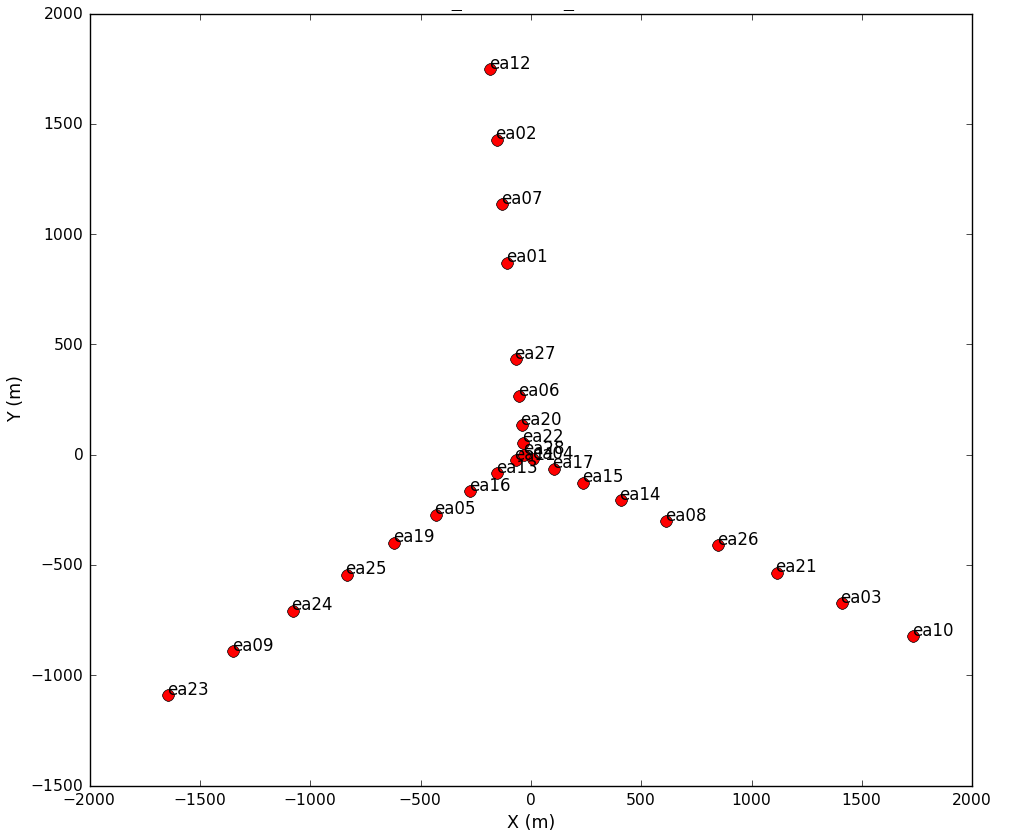
\includegraphics[width=\linewidth, trim={18px 19px 18px 18px}, clip]{./chapters/01.intro/img/antennas.png}
		\caption{Antenna Configuration}
	\end{subfigure}
	\begin{subfigure}[b]{0.28\linewidth}
		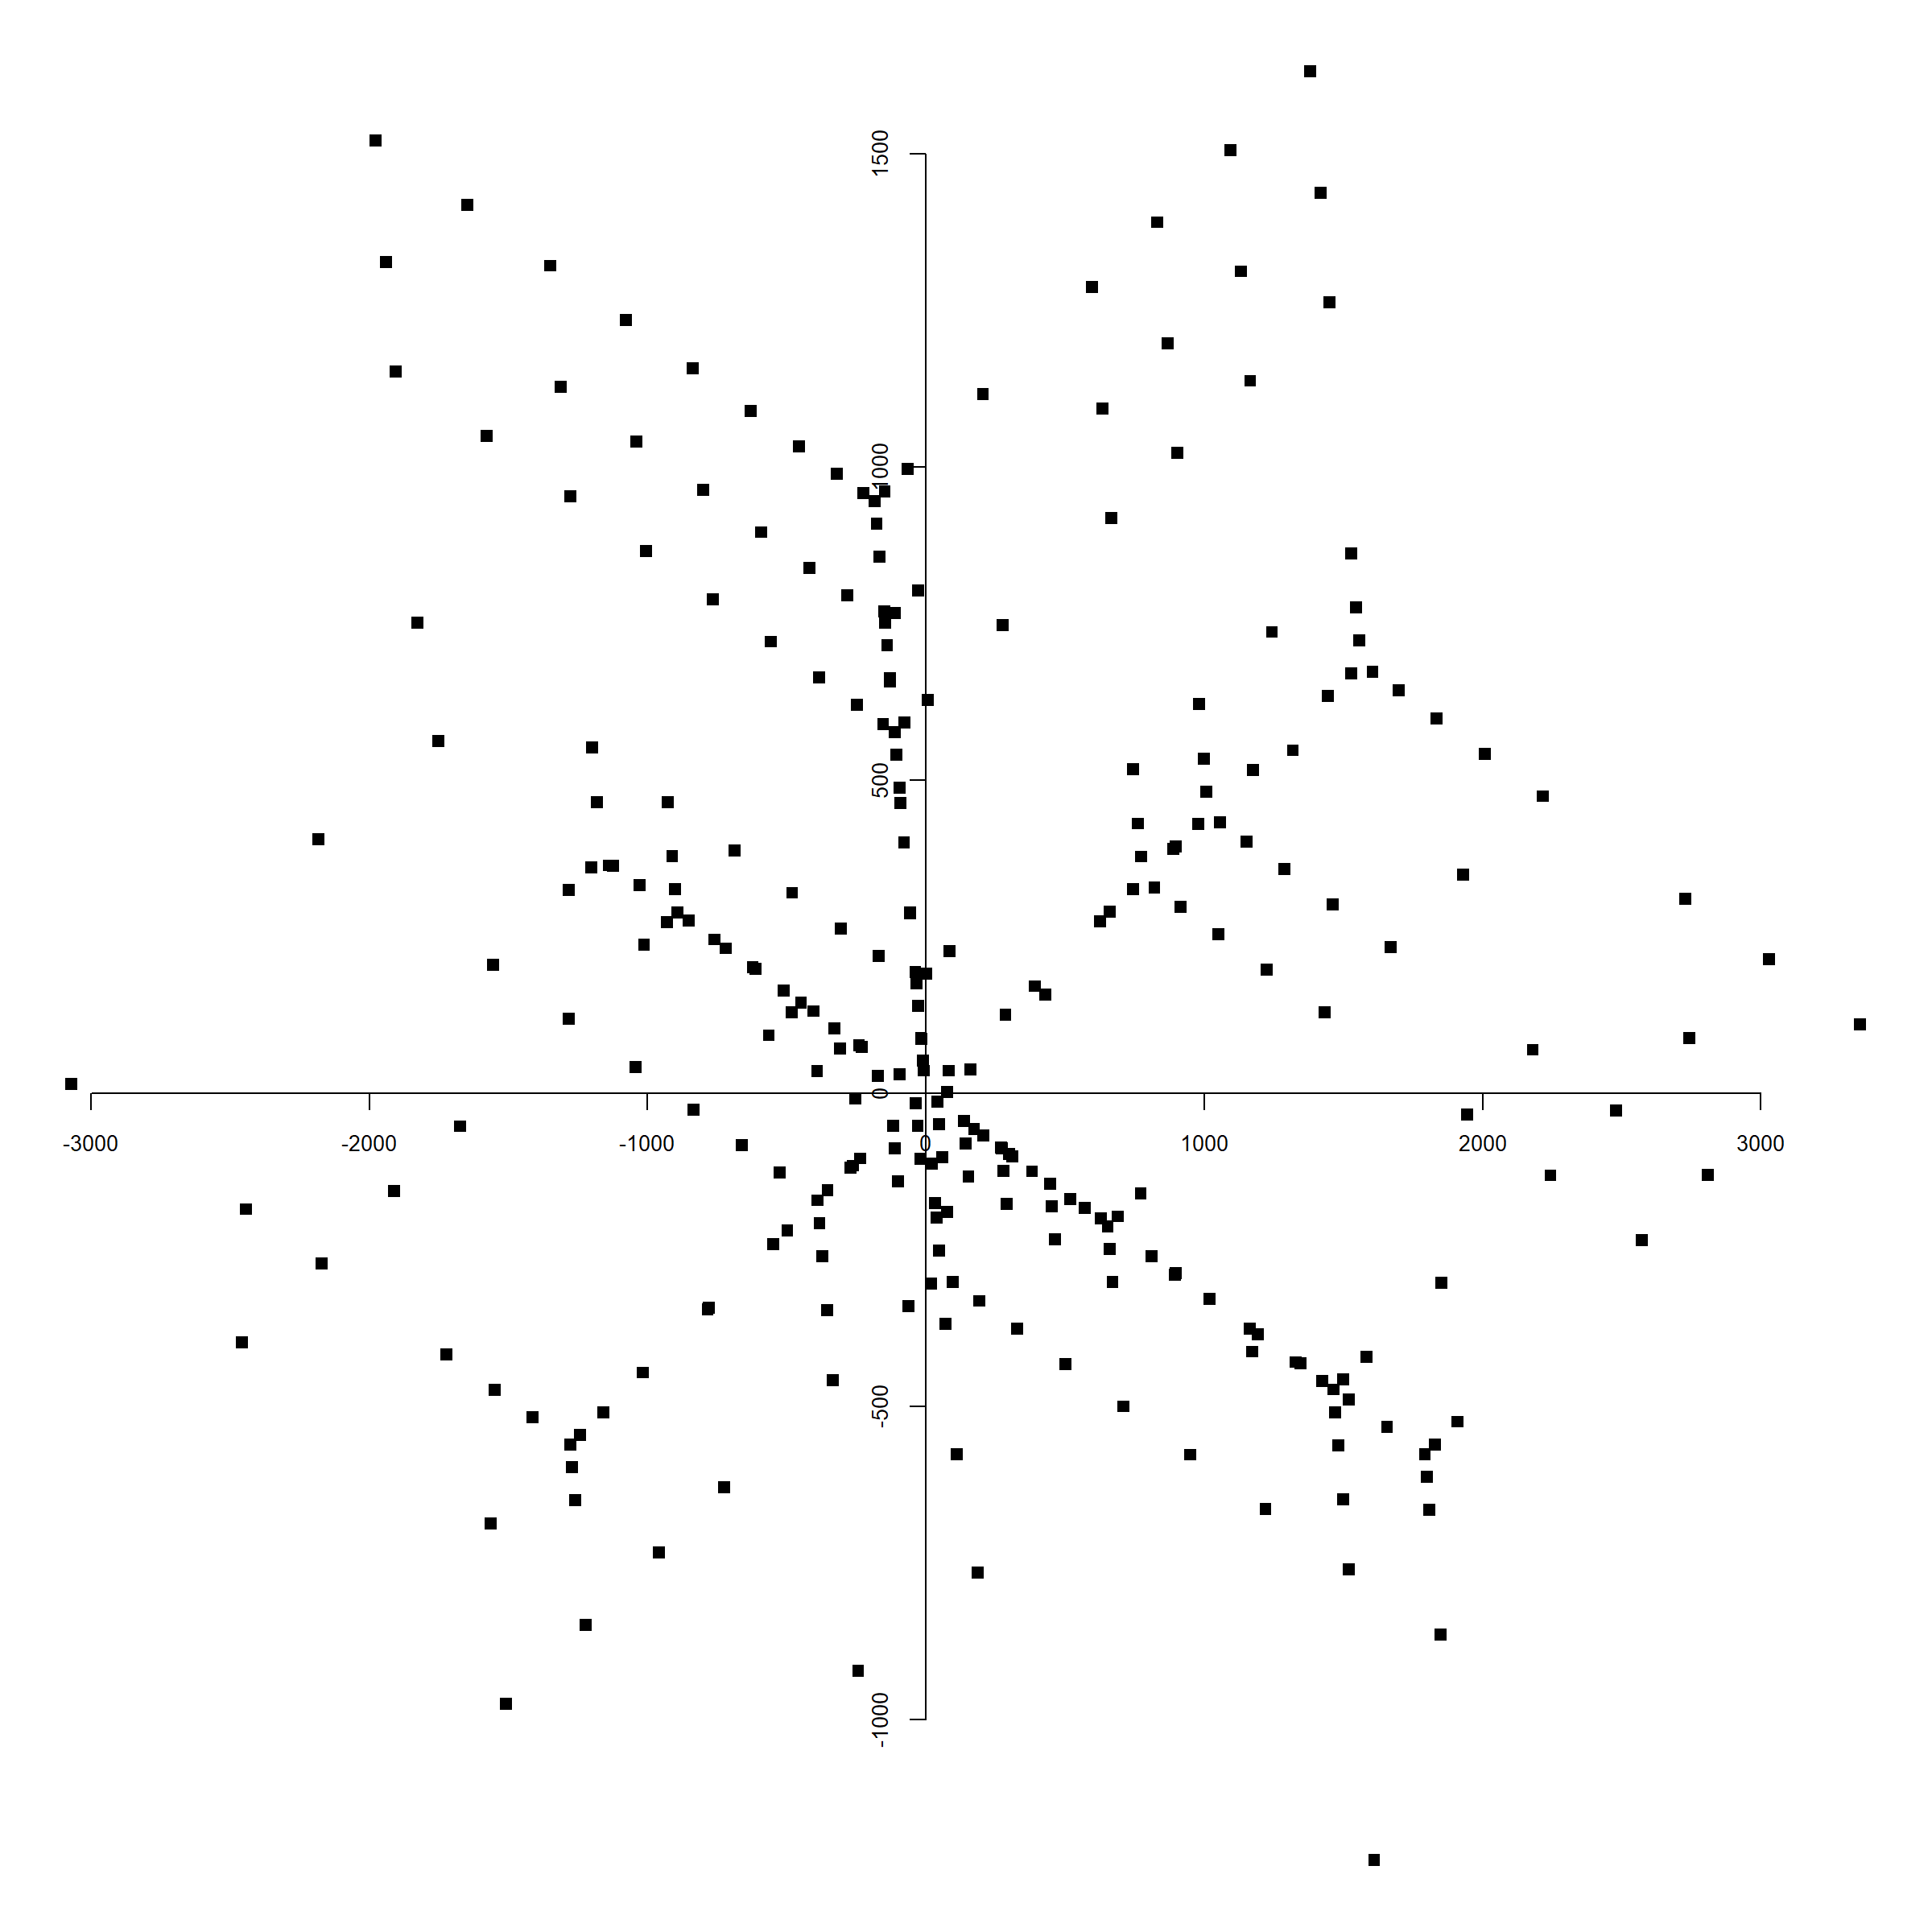
\includegraphics[width=\linewidth, trim={18px 19px 18px 18px}, clip]{./chapters/01.intro/img/uv.png}
		\caption{UV-Space}
	\end{subfigure}
	\begin{subfigure}[b]{0.28\linewidth}
		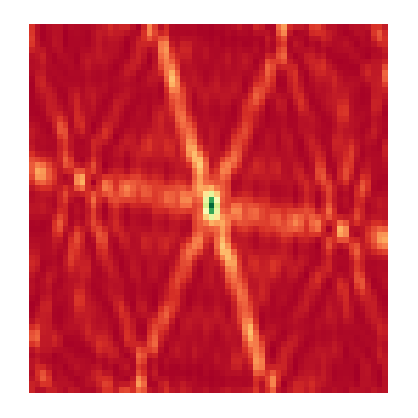
\includegraphics[width=\linewidth, trim={18px 19px 18px 18px}, clip]{./chapters/01.intro/img/psf.png}
		\caption{PSF}
	\end{subfigure}

	\begin{subfigure}[b]{0.28\linewidth}
		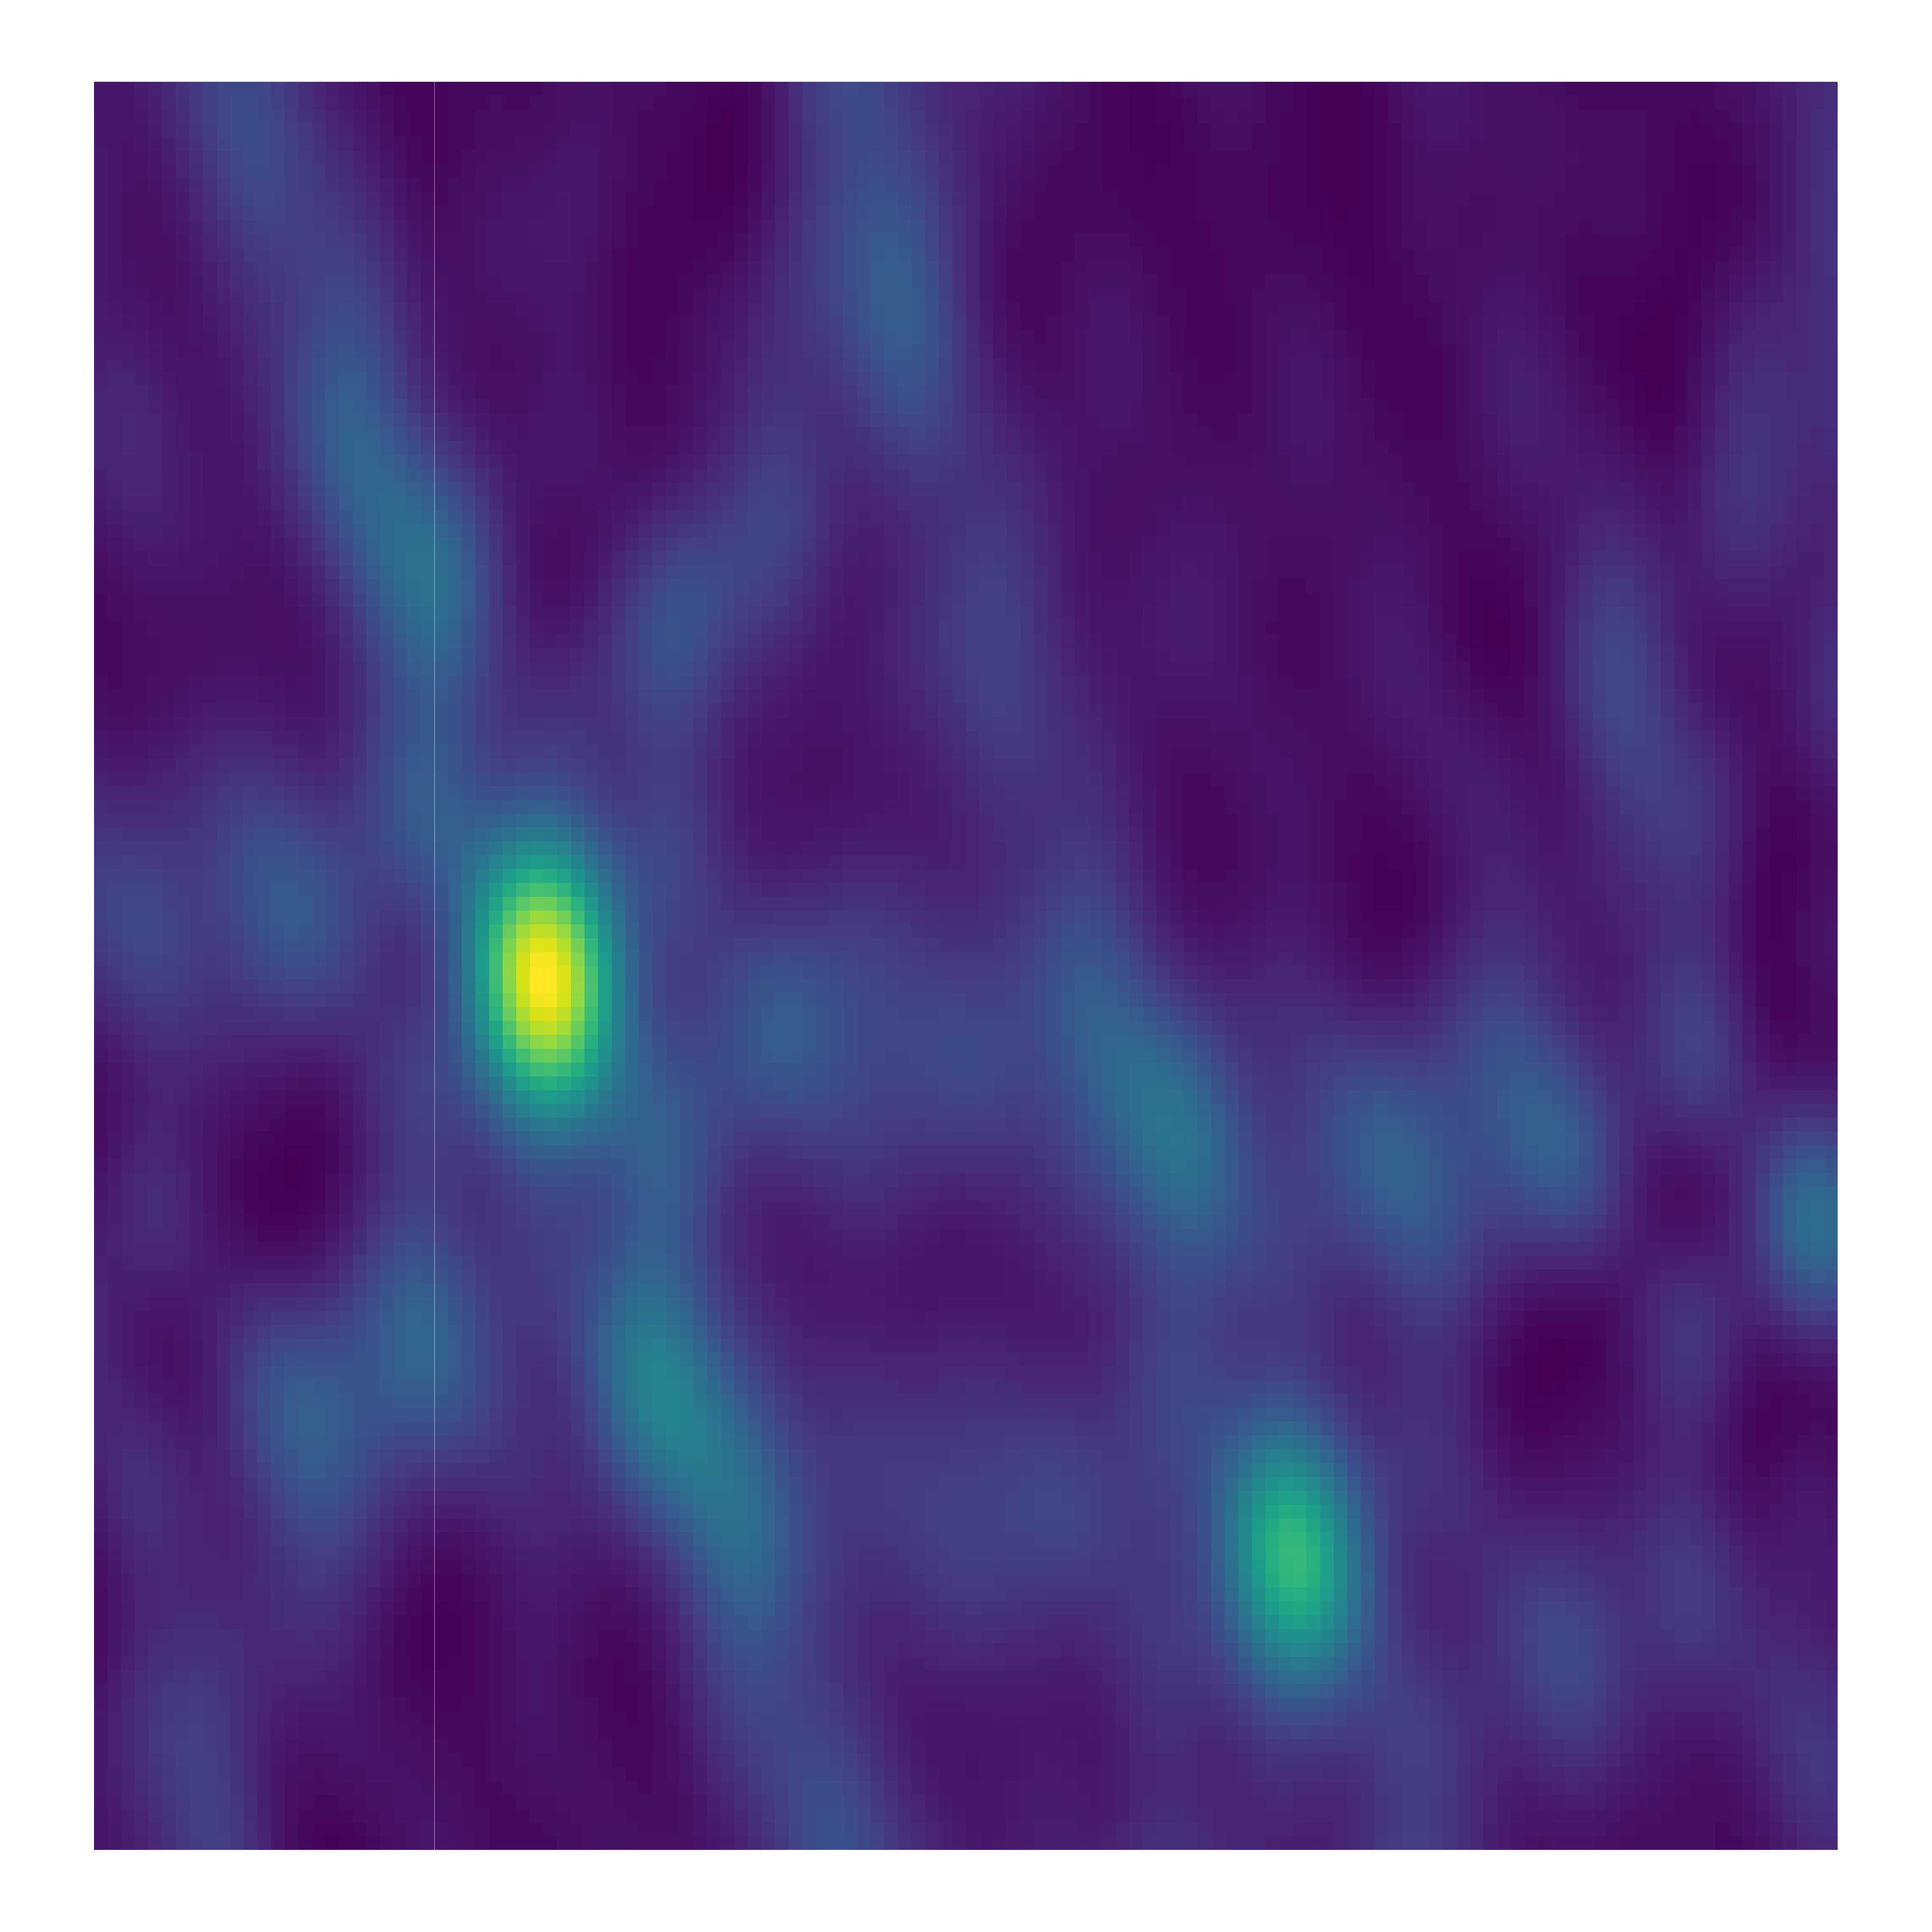
\includegraphics[width=\linewidth, trim={18px 19px 18px 18px}, clip]{./chapters/01.intro/img/dirty_image.png}
		\caption{dirty image}
	\end{subfigure}
	\begin{subfigure}[b]{0.28\linewidth}
		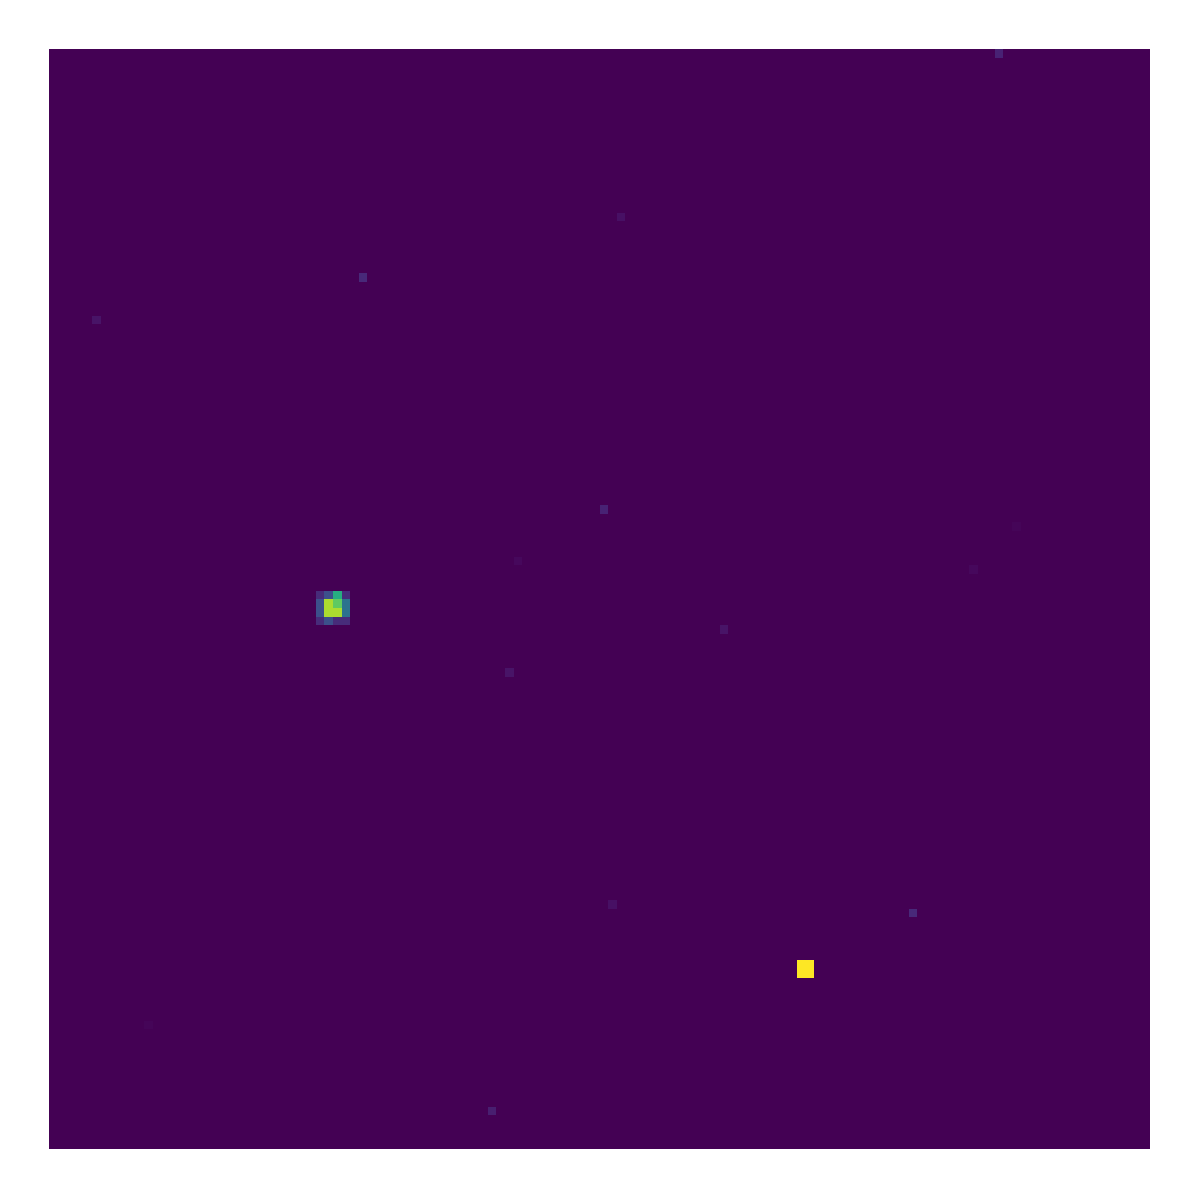
\includegraphics[width=\linewidth, trim={18px 19px 18px 18px}, clip]{./chapters/01.intro/img/true_image.png}
		\caption{true image}
	\end{subfigure}
	\caption{Inverse Problem example for VLA: Retrieve the true image when only PSF and dirty image are known}
	\label{intro:measurement_problem}
\end{figure}

The Inverse Problem is now to remove the artefacts of the interferometer and retrieve the true image. The effects of the undersampling can be modeled by a Point Spread Function (PSF). The interferometer sees the true image of the sky, but due to undersampling it gets convolved with a PSF, resulting in the dirty image.  More formally, we try to find a solution $x$ for equation \eqref{intro:eq:deconvolve}, where only the PSF and $I_{dirty}$ are known. This problem is ill-posed: it may have multiple solutions, and a small change in the $I_{dirty}$ or the PSF may result in large changes in $x$. Furthermore, the whole problem gets corrupted by noise.

\begin{equation}\label{intro:eq:deconvolve}
x \star  PSF + N = I_{dirty} 
\end{equation}

The PSF is surprisingly easy to calculate. The Fourier Transformed PSF equals the sampling pattern in UV-Space. Remember that a convolution in image space is a multiplication in Fourier. The effects of under-sampling in image space are a convolution with the PSF. In the Fourier space it is masking all components other than the measured ones. From the Antenna Configuration we can infer the masking matrix $M$ in UV-Space. Calculating the Inverse Fourier Transform of $M$ results in the PSF.


\subsection{Deconvolution with CLEAN}
In each iteration of CLEAN, it searches the highest peak of the dirty image and removing a fraction of the PSF at that point. It stops until the next highest peak is below a threshold, or if the maximum number of iterations was reached. The fraction of the PSF, threshold and number of iterations are all tunable by the user. State of the art implementations expose even more parameters. The reconstruction quality depends on the chosen parameters and require extensive user input.

%Convolved with the primary beam
CLEAN does not solve the deconvolution problem \eqref{intro:eq:deconvolve} directly. Instead, it greedily minimizes the objective \eqref{intro:eq:clean}. It is easy to see that if CLEAN minimizes the objective to zero, it has found a solution to the original deconvolution problem in a noiseless environment.

\begin{equation}\label{intro:eq:clean}
\underset{x}{minimize} \: \left \| I_{dirty} - x \star PSF \right \|_2^2
\end{equation}

Since the original problem is ill-posed, the objective \eqref{intro:eq:clean} may have several zero points. In practice, CLEAN is stopped before it reaches zero. The addition of noise can add spurious peaks in the dirty image. By stopping early, CLEAN regularizes the objective. It assumes only a limited number of point sources exist in the image. The larger the magnitude of the peak, the more likely it is to be a real point source.

In short, CLEAN does a greedy approximation of the deconvolution problem, and assumes the resulting image consists out of a few point sources. The question remains, how close the CLEAN approximation is to the true image? If the true image consists out of a few point sources, CLEAN produces a good approximation. Extended emissions however are harder for CLEAN to reproduce. The peak of extended sources is lower than that of point sources. It is harder for CLEAN to distinguish extended sources from noise.

The CLEAN regularization scheme is not ideal for extended sources. Ideally another way of regularization would be chosen for extended emissions, but the regularization is a fixed part of the CLEAN algorithm.


\subsection{From CLEAN to Compressed Sensing}
In the Compressed Sensing Framework, an approach is split into three separate parts:
\begin{itemize}
	\item An objective with a data and regularization term
	\item A prior $P$ in which the signal can be sparsely represented.
	\item An optimization algorithm that is suited for the objective.
\end{itemize}


The fra
To demonstrate the flexibility of the Compressed Sensing Framework, we convert CLEAN into a Compressed Sensing approach. First we add a regularization term to \eqref{intro:eq:clean} and arrive at the new objective \eqref{intro:eq:csclean}. The objective contains the old CLEAN data term and a new regularization term. The data term forces the reconstruction to be close to the measurement, while the regularization term forces the reconstruction to be plausible. $\lambda$ models the expected noise in the problem. Note that the zero norm $\left \| Px \right \|_0$ acts as an indicator function. 

\begin{equation}\label{intro:eq:csclean}
	\underset{x}{minimize} \: \left \| D_{dirty} - x \star PSF \right \|_2^2 \: + \: \lambda \left \| Px \right \|_0
\end{equation}

Now $P$ that models the same regularization scheme. CLEAN assumes the $x$ contains a few point sources. In Compressed Sensing terminology, it assumes $x$ is sparse in image space. Since $x$ is already an image, the Prior $P$ in Compressed Sensing CLEAN is the identity matrix. 

CLEAN uses a greedy optimization scheme. In every iteration, CLEAN searches the highest peak in the dirty image. Matching Pursuit is a greedy optimization scheme for $L0$ objectives like our Compressed Sensing CLEAN \eqref{intro:eq:csclean}.





Both versions of CLEAN produce the same result, but we are getting rid of the tunable parameters in favour of a single $\lambda$. There exist schemes that estimate the correct $\lambda$ for a given problem.

In the noisy environment the true image may not be located at a minimum of the CLEAN objective \eqref{intro:eq:clean}. The Compressed Sensing objective is guaranteed to have a unique global minimum and the true image is guaranteed to be there if:
\begin{itemize}
	\item The Prior models our signal well enough
	\item Enough samples are available. 
\end{itemize}

How many samples are needed? Interestingly enough, we do not need the Nyquist-Shannon rate. It depends on the prior. 

Same as clean, but now we have a global optimization scheme, the regularization is explicit and replaceable.

The important questions are: In an undersampled, noisy environment, does the new objective \eqref{intro:eq:csclean} have a global minimum? What is the chances that the minimum is equal to the true image? It turns out that even though we have fewer samples than the Nyquist-Shannon Theorem requires, we can guarantee a global minimum and that the minimum is equal to the true image, if we have enough prior knowledge $P$ about the signal. How we model the signal and by extend, what $P$ we choose is essential for Compressed Sensing


The data term is for small Field of View imaging, it can be modified to solve the wide Field of View problem.





